\documentclass{article}
\usepackage[submission]{../colm2026_conference}
\usepackage[utf8]{inputenc}
\usepackage[T1]{fontenc}
\usepackage{microtype}
\usepackage{hyperref}
\usepackage{url}
\usepackage{booktabs}
\usepackage{longtable}
\usepackage{array}
\usepackage{graphicx}
\usepackage{amsmath,amssymb}
\usepackage{caption}
\usepackage{lineno}

\definecolor{darkblue}{rgb}{0, 0, 0.5}
\hypersetup{
  colorlinks=true,
  citecolor=darkblue,
  linkcolor=darkblue,
  urlcolor=darkblue,
  pdfauthor={Anonymous},
  pdftitle={When Byte-Scale Model Communication Should Be Text},
  pdfsubject={COLM 2026 submission},
  pdfkeywords={},
  pdfcreator={LaTeX},
  pdfproducer={}
}
\urlstyle{same}
\graphicspath{{figures/}}
\setkeys{Gin}{width=0.92\linewidth,height=0.27\textheight,keepaspectratio}
\setcounter{secnumdepth}{2}
\newcommand{\tightlist}{\setlength{\itemsep}{0pt}\setlength{\parskip}{0pt}}

\title{When Byte-Scale Model Communication Should Be Text\\\large A Controlled Negative for Discrete No-Text Packets}
\author{Anonymous Authors}

\begin{document}
\ifcolmsubmission
\linenumbers
\fi
\maketitle

\begin{abstract}
LatentWire asks whether a source model can send a small no-text packet
that improves a receiver model beyond ordinary score and text baselines.
The answer for the completed discrete, byte-scale regime is a bounded
negative. One-way score and residual packets do not beat
source-index/confidence controls on the held-out aggregate, and the
powered score ladder explains why: apparent source information drops
from \(2.098527\) bits to \(0.281933\) bits after conditioning
on receiver evidence. The strongest discrete-evidence escape fails in
the opposite direction: when the same exact symbolic evidence is exposed
as a visible 2-byte public code, it reaches \(1.000\) accuracy
versus \(0.775\) for the matched learned packet, a \(+0.225\)
advantage with 95\% CI \texttt{{[}0.192188,\ 0.257812{]}}. The last
cheap privacy-bottleneck escape also fails: the privacy-bottleneck
escape is utility is identity leakage, with the current
packet at utility/leakage \(0.875/1.000\) and the best bottleneck
at only \(0.602339/0.602339\). We contribute a reusable
falsification ladder showing that discrete low-byte no-text packet wins
vanish under source-index, equal-byte visible evidence, and
privacy-bottleneck controls.
\end{abstract}

\hypertarget{claim-boundary-box}{%
\subsection{Claim-Boundary Box}\label{claim-boundary-box}}

\begingroup\small
\begin{longtable}[]{@{}lll@{}}
\toprule
\begin{minipage}[b]{0.30\columnwidth}\raggedright
Supported\strut
\end{minipage} & \begin{minipage}[b]{0.30\columnwidth}\raggedright
Unsupported\strut
\end{minipage} & \begin{minipage}[b]{0.30\columnwidth}\raggedright
Future-only\strut
\end{minipage}\tabularnewline
\midrule
\endhead
\begin{minipage}[t]{0.30\columnwidth}\raggedright
Score-like source packets are bounded negative under
source-index/confidence controls.\strut
\end{minipage} & \begin{minipage}[t]{0.30\columnwidth}\raggedright
A deployable-positive claim is unsupported.\strut
\end{minipage} & \begin{minipage}[t]{0.30\columnwidth}\raggedright
Continuous dense cache/state transfer may still work, but it is outside
this byte-scale discrete packet result.\strut
\end{minipage}\tabularnewline
\begin{minipage}[t]{0.30\columnwidth}\raggedright
Exact discrete evidence is text-capturable under the same byte budget in
the local cache.\strut
\end{minipage} & \begin{minipage}[t]{0.30\columnwidth}\raggedright
the privacy-bottleneck escape is not a privacy positive; it remains
utility is identity leakage.\strut
\end{minipage} & \begin{minipage}[t]{0.30\columnwidth}\raggedright
A reviewed neural privacy bottleneck would need matched
visible/anonymized text controls.\strut
\end{minipage}\tabularnewline
\begin{minipage}[t]{0.30\columnwidth}\raggedright
Answer-aware oracle ceilings are rejected as leakage or gap-to-perfect
measurements.\strut
\end{minipage} & \begin{minipage}[t]{0.30\columnwidth}\raggedright
No cross-family, dense-cache, native GPU, or systems-speed claim is
made.\strut
\end{minipage} & \begin{minipage}[t]{0.30\columnwidth}\raggedright
Stronger generated-candidate reranking remains possible only with
gold-blind verifier/source/target scores.\strut
\end{minipage}\tabularnewline
\bottomrule
\end{longtable}
\endgroup

\hypertarget{introduction}{%
\subsection{1. Introduction}\label{introduction}}

Small model-to-model messages are attractive because they promise
communication without exposing full reasoning traces. The hard question
is not whether a helper model knows something useful. It is whether a
byte-scale no-text packet conveys information that the receiver cannot
already recover from its own scores, the source identity, or an
equal-byte visible code.

This campaign originally searched for a positive LatentWire method. The
result is a stronger and more useful boundary: the discrete evidence
that makes a packet useful is visible-code capturable, while score-like
residual signals mostly disappear after receiver conditioning. The paper
therefore argues for a conservative standard for future model
communication work: the relevant delta is not improvement over
target-only, but improvement beyond source-index, source-confidence,
equal-byte text, wrong-row, and destructive controls.

The contribution is deliberately positive in the bounded-negative sense.
It gives future latent-communication papers a falsification ladder:
source-index and confidence first, equal-byte visible evidence next,
then wrong-row/destructive controls and privacy-leakage probes. A packet
that cannot survive that ladder should not be described as deployable
communication.

Contributions:

\begin{enumerate}
\def\labelenumi{\arabic{enumi}.}
\item
  A controlled bounded negative for deployable score/residual packets.
  On the held-out aggregate with \(381\) rows, the deployable score
  packet is \(-0.023622\) below source-index/confidence with CI
  \texttt{{[}-0.060367,\ 0.013123{]}}. On the powered dev/gate ladder
  with \(1500\) scored rows and \(359\) gate rows, the current
  deployable packet is \(-0.013928\) below the best score baseline
  with CI \texttt{{[}-0.050139,\ 0.022284{]}}.
\item
  A mechanism for the negative result. Source scores contain
  \(2.098527\) bits before receiver conditioning, but only
  \(0.281933\) bits after conditioning on receiver evidence (Figure
  1).
\item
  A direct exact-discrete evidence test. On \(640\) model-helper
  rows over \(160\) unique examples, a matched model packet reaches
  \(0.775\) accuracy, while the exact same symbolic evidence
  serialized as visible public code reaches \(1.000\) (Figure 3).
  Random, shuffled, answer-only, and target-only controls remain at
  \(0.250\).
\item
  A final cheap privacy escape test. the privacy-bottleneck escape
  cannot preserve current-packet utility while hiding source/evidence
  identity (Figure 4).
\end{enumerate}

\begin{figure}
\centering
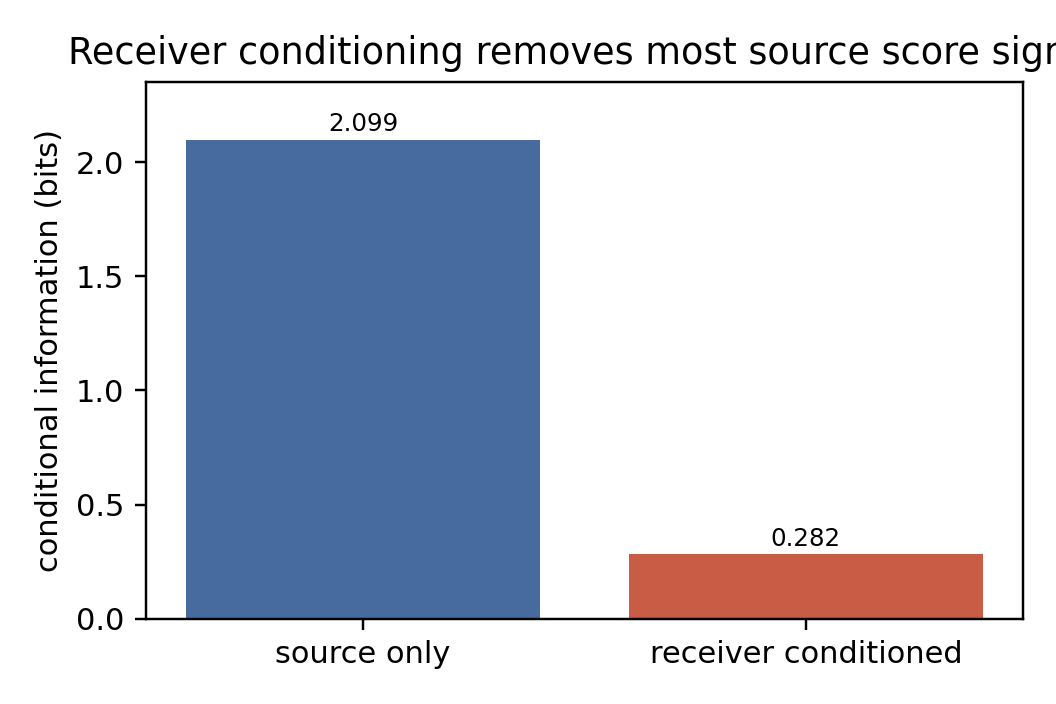
\includegraphics{figures/receiver_conditioning_bits.png}
\caption{Receiver conditioning bits}
\end{figure}

Figure 1: Powered cached support: the source-score signal largely
disappears once receiver evidence is included.

\hypertarget{experimental-setup-and-regimes}{%
\subsection{2. Experimental Setup And
Regimes}\label{experimental-setup-and-regimes}}

The results below are not all from one dataset. That is intentional:
each row is a different escape hatch with its own control surface.

\begingroup\small
\begin{longtable}[]{@{}lllll@{}}
\toprule
\begin{minipage}[b]{0.17\columnwidth}\raggedright
Result block\strut
\end{minipage} & \begin{minipage}[b]{0.17\columnwidth}\raggedright
Dataset/cache\strut
\end{minipage} & \begin{minipage}[b]{0.17\columnwidth}\raggedright
Model or endpoint role\strut
\end{minipage} & \begin{minipage}[b]{0.17\columnwidth}\raggedright
Classes / task shape\strut
\end{minipage} & \begin{minipage}[b]{0.17\columnwidth}\raggedright
n and caveat\strut
\end{minipage}\tabularnewline
\midrule
\endhead
\begin{minipage}[t]{0.17\columnwidth}\raggedright
Held-out score/WZ null\strut
\end{minipage} & \begin{minipage}[t]{0.17\columnwidth}\raggedright
MMLU-Pro aggregate from the one-way deployable packet closeout\strut
\end{minipage} & \begin{minipage}[t]{0.17\columnwidth}\raggedright
source-score packet to target receiver\strut
\end{minipage} & \begin{minipage}[t]{0.17\columnwidth}\raggedright
multiple-choice; weak-signal regime\strut
\end{minipage} & \begin{minipage}[t]{0.17\columnwidth}\raggedright
\(381\) aggregate held-out rows; raw held-out rows not
packaged\strut
\end{minipage}\tabularnewline
\begin{minipage}[t]{0.17\columnwidth}\raggedright
Powered score ladder\strut
\end{minipage} & \begin{minipage}[t]{0.17\columnwidth}\raggedright
MMLU-Pro dev/gate score surface\strut
\end{minipage} & \begin{minipage}[t]{0.17\columnwidth}\raggedright
Qwen2.5-0.5B source to Qwen3-0.6B target\strut
\end{minipage} & \begin{minipage}[t]{0.17\columnwidth}\raggedright
multiple-choice score sketches\strut
\end{minipage} & \begin{minipage}[t]{0.17\columnwidth}\raggedright
\(1500\) scored dev/gate rows; \(359\) gate rows\strut
\end{minipage}\tabularnewline
\begin{minipage}[t]{0.17\columnwidth}\raggedright
the receiver-query escape query packet\strut
\end{minipage} & \begin{minipage}[t]{0.17\columnwidth}\raggedright
same powered dev/gate surface\strut
\end{minipage} & \begin{minipage}[t]{0.17\columnwidth}\raggedright
query/reply packet and ablations\strut
\end{minipage} & \begin{minipage}[t]{0.17\columnwidth}\raggedright
multiple-choice\strut
\end{minipage} & \begin{minipage}[t]{0.17\columnwidth}\raggedright
\(359\) gate rows\strut
\end{minipage}\tabularnewline
\begin{minipage}[t]{0.17\columnwidth}\raggedright
Exact discrete evidence\strut
\end{minipage} & \begin{minipage}[t]{0.17\columnwidth}\raggedright
test-log/code-helper cache\strut
\end{minipage} & \begin{minipage}[t]{0.17\columnwidth}\raggedright
helper rows over a finite symbolic evidence signature\strut
\end{minipage} & \begin{minipage}[t]{0.17\columnwidth}\raggedright
4-way candidate choice\strut
\end{minipage} & \begin{minipage}[t]{0.17\columnwidth}\raggedright
\(640\) model-helper rows, but only \(160\) unique
examples\strut
\end{minipage}\tabularnewline
\begin{minipage}[t]{0.17\columnwidth}\raggedright
the privacy-bottleneck escape privacy bottleneck\strut
\end{minipage} & \begin{minipage}[t]{0.17\columnwidth}\raggedright
candidate-conditioned packet-builder cache\strut
\end{minipage} & \begin{minipage}[t]{0.17\columnwidth}\raggedright
cached feature selector/adversary proxy\strut
\end{minipage} & \begin{minipage}[t]{0.17\columnwidth}\raggedright
4-way candidate/evidence atoms\strut
\end{minipage} & \begin{minipage}[t]{0.17\columnwidth}\raggedright
\(512\) matched rows; proxy only\strut
\end{minipage}\tabularnewline
\bottomrule
\end{longtable}
\endgroup

This mapping matters because the target-only baseline is \(0.194\)
in the held-out MMLU-Pro aggregate but \(0.250\) in the 4-way
exact-evidence cache. Those are different tasks, not inconsistent
measurements.

Claim provenance is summarized in the text and figures.

\hypertarget{falsification-ladder}{%
\subsection{3. Falsification Ladder}\label{falsification-ladder}}

The central asset of this paper is not a single negative row. It is a
ladder of increasingly plausible escapes, each killed or parked by a
concrete hard baseline.

\begingroup\small
\begin{longtable}[]{@{}llll@{}}
\toprule
\begin{minipage}[b]{0.22\columnwidth}\raggedright
Escape\strut
\end{minipage} & \begin{minipage}[b]{0.22\columnwidth}\raggedright
What it would have shown\strut
\end{minipage} & \begin{minipage}[b]{0.22\columnwidth}\raggedright
Result\strut
\end{minipage} & \begin{minipage}[b]{0.22\columnwidth}\raggedright
Controlling baseline / audit\strut
\end{minipage}\tabularnewline
\midrule
\endhead
\begin{minipage}[t]{0.22\columnwidth}\raggedright
Score/WZ one-way packet\strut
\end{minipage} & \begin{minipage}[t]{0.22\columnwidth}\raggedright
A deployable low-byte source residual beats source-score controls\strut
\end{minipage} & \begin{minipage}[t]{0.22\columnwidth}\raggedright
held-out delta \(-0.023622\), CI
\texttt{{[}-0.060367,\ 0.013123{]}}, \texttt{n=381}\strut
\end{minipage} & \begin{minipage}[t]{0.22\columnwidth}\raggedright
source-index+confidence\strut
\end{minipage}\tabularnewline
\begin{minipage}[t]{0.22\columnwidth}\raggedright
Powered score ladder\strut
\end{minipage} & \begin{minipage}[t]{0.22\columnwidth}\raggedright
Receiver has residual headroom after source scores\strut
\end{minipage} & \begin{minipage}[t]{0.22\columnwidth}\raggedright
current packet delta \(-0.013928\), CI
\texttt{{[}-0.050139,\ 0.022284{]}}, gate \texttt{n=359}\strut
\end{minipage} & \begin{minipage}[t]{0.22\columnwidth}\raggedright
best equal-byte score/source baseline\strut
\end{minipage}\tabularnewline
\begin{minipage}[t]{0.22\columnwidth}\raggedright
the damage-avoidance escape damage-avoidance trust packet\strut
\end{minipage} & \begin{minipage}[t]{0.22\columnwidth}\raggedright
Packet improves repair without copying source answer\strut
\end{minipage} & \begin{minipage}[t]{0.22\columnwidth}\raggedright
killed in Stage-1: matched packet mostly equals source-selected answer
and damage avoidance fails\strut
\end{minipage} & \begin{minipage}[t]{0.22\columnwidth}\raggedright
source-index/source-selected metadata\strut
\end{minipage}\tabularnewline
\begin{minipage}[t]{0.22\columnwidth}\raggedright
the receiver-query escape receiver-query packet\strut
\end{minipage} & \begin{minipage}[t]{0.22\columnwidth}\raggedright
Two-way query/reply creates new usable evidence\strut
\end{minipage} & \begin{minipage}[t]{0.22\columnwidth}\raggedright
delta \(-0.022284\), CI \texttt{{[}-0.055710,\ 0.011142{]}},
\texttt{n=359}\strut
\end{minipage} & \begin{minipage}[t]{0.22\columnwidth}\raggedright
source-index+confidence; query-only/reply-only ablations\strut
\end{minipage}\tabularnewline
\begin{minipage}[t]{0.22\columnwidth}\raggedright
Exact discrete evidence\strut
\end{minipage} & \begin{minipage}[t]{0.22\columnwidth}\raggedright
Opaque packet carries symbolic evidence better than visible code\strut
\end{minipage} & \begin{minipage}[t]{0.22\columnwidth}\raggedright
visible exact code \(1.000\) vs packet \(0.775\); delta
\(+0.225\), CI \texttt{{[}0.192188,\ 0.257812{]}}\strut
\end{minipage} & \begin{minipage}[t]{0.22\columnwidth}\raggedright
equal-byte public code; random/shuffled/answer-only controls at
\(0.250\)\strut
\end{minipage}\tabularnewline
\begin{minipage}[t]{0.22\columnwidth}\raggedright
the privacy-bottleneck escape privacy bottleneck\strut
\end{minipage} & \begin{minipage}[t]{0.22\columnwidth}\raggedright
Utility can be preserved while hiding source/evidence identity\strut
\end{minipage} & \begin{minipage}[t]{0.22\columnwidth}\raggedright
best bottleneck utility/leakage \(0.602339/0.602339\); current
packet \(0.875/1.000\)\strut
\end{minipage} & \begin{minipage}[t]{0.22\columnwidth}\raggedright
same-byte visible code and adaptive anonymized text\strut
\end{minipage}\tabularnewline
\begin{minipage}[t]{0.22\columnwidth}\raggedright
C2C/KVComm local checks\strut
\end{minipage} & \begin{minipage}[t]{0.22\columnwidth}\raggedright
Dense/cache anchors become byte-scale method evidence\strut
\end{minipage} & \begin{minipage}[t]{0.22\columnwidth}\raggedright
anchor only; answer packets leak answer text or tie deterministic
controls\strut
\end{minipage} & \begin{minipage}[t]{0.22\columnwidth}\raggedright
zero-source, teacher/candidate, deterministic packet controls\strut
\end{minipage}\tabularnewline
\begin{minipage}[t]{0.22\columnwidth}\raggedright
rerank/fuser oracle ceilings\strut
\end{minipage} & \begin{minipage}[t]{0.22\columnwidth}\raggedright
Rerank/fuser ceilings imply deployable latent methods\strut
\end{minipage} & \begin{minipage}[t]{0.22\columnwidth}\raggedright
rejected as oracle-only or setup-blocked; gold-aware ceilings are not
claims\strut
\end{minipage} & \begin{minipage}[t]{0.22\columnwidth}\raggedright
gold-leakage audit and equal-byte text controls\strut
\end{minipage}\tabularnewline
\bottomrule
\end{longtable}
\endgroup

The full audit provenance is retained internally; the submitted paper
reports only the claim-bearing summaries.

\hypertarget{results}{%
\subsection{4. Results}\label{results}}

\hypertarget{deployable-packets-do-not-beat-source-index-confidence}{%
\subsubsection{4.1 Deployable Packets Do Not Beat Source-Index
Confidence}\label{deployable-packets-do-not-beat-source-index-confidence}}

\begin{figure}
\centering
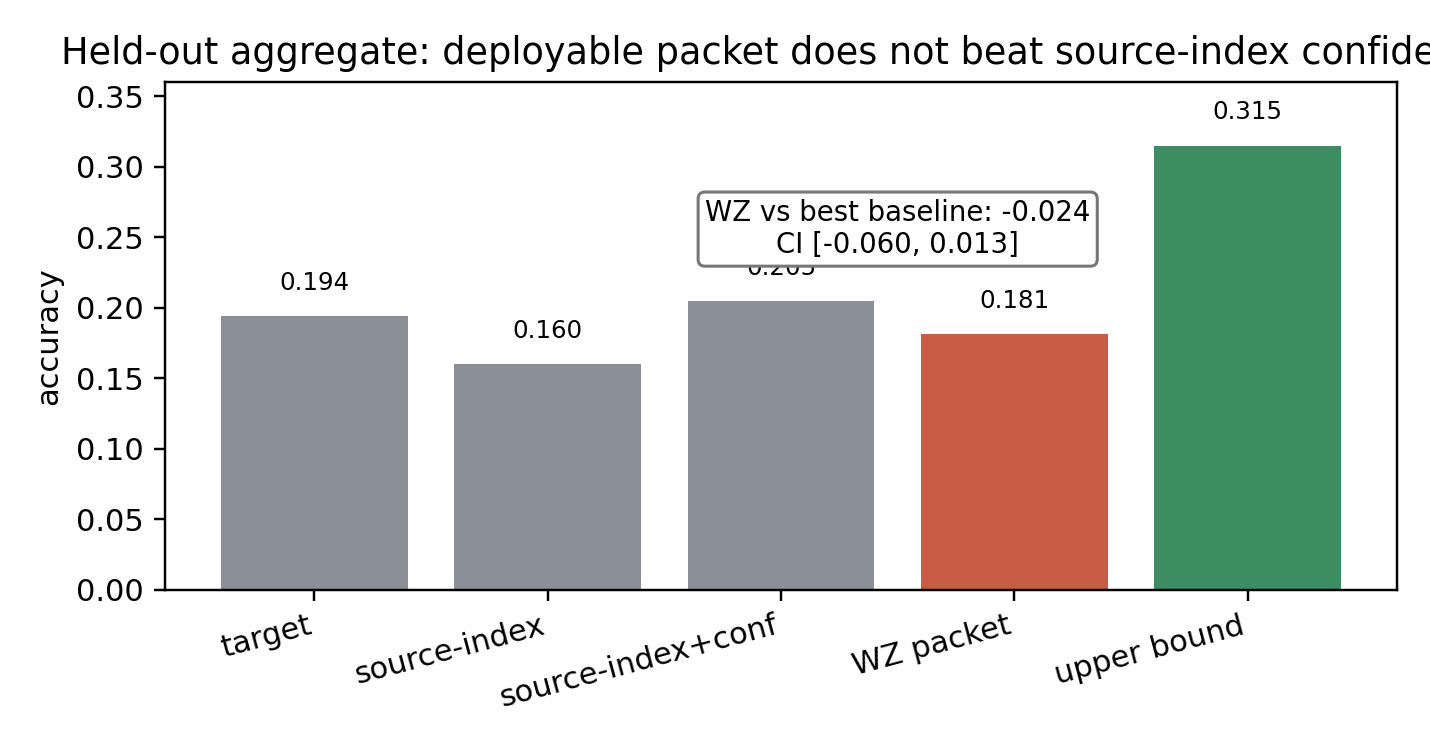
\includegraphics{figures/heldout_source_index_null.png}
\caption{Held-out source-index null}
\end{figure}

Figure 2: On the held-out aggregate, the deployable packet does not beat
the source-index/confidence baseline. The source+target-at-encoder upper
bound is positive but non-deployable.

The held-out aggregate shows the exact boundary. Target-only accuracy is
\(0.194226\), source-index+confidence is \(0.204724\), and the
deployable WZ packet is \(0.181102\). The source+target-at-encoder
upper bound reaches \(0.314961\), so the experiment is not merely
noise. The problem is deployability: the useful signal appears when the
encoder has target evidence, not in the allowed source-only low-byte
packet.

\hypertarget{receiver-conditioning-explains-the-null}{%
\subsubsection{4.2 Receiver Conditioning Explains The
Null}\label{receiver-conditioning-explains-the-null}}

The powered ladder estimates \(2.098527\) bits of source-score
information before receiver conditioning and \(0.281933\) bits
afterward. Same-family models on shared multiple-choice tasks often fail
and succeed for overlapping reasons. A source packet can therefore
appear useful until the receiver's own evidence and the source identity
are included as baselines.

A natural objection is that the held-out task is a weak-signal regime:
the receiver's own accuracy (\(0.194\)) and the
source-index+confidence baseline (\(0.205\)) sit only modestly
above chance, so a small negative delta could reflect a task no model
solves rather than a ceiling on packet utility. Two pieces of evidence
rule this out. First, information is demonstrably present: the
source+target-at-encoder upper bound reaches \(0.315\), far above
every deployable condition, so the packet's failure is one of
deployability, not of available signal. Second, the
receiver-conditioning estimate is base-rate-independent: the
source-score signal collapses from \(2.10\) to \(0.28\) bits
once the receiver's own evidence is conditioned on, measuring redundancy
directly rather than through task accuracy. The negative therefore
reflects that a source-only low-byte packet conveys little the receiver
does not already hold, regardless of how hard the underlying task is.

This result also explains why source-only oracle gaps are not enough. A
positive source+target-at-encoder upper bound says there is information
in the joint state; it does not say a deployable source-only byte packet
transmits it.

\hypertarget{exact-discrete-evidence-is-better-sent-as-text}{%
\subsubsection{4.3 Exact Discrete Evidence Is Better Sent As
Text}\label{exact-discrete-evidence-is-better-sent-as-text}}

\begin{figure}
\centering
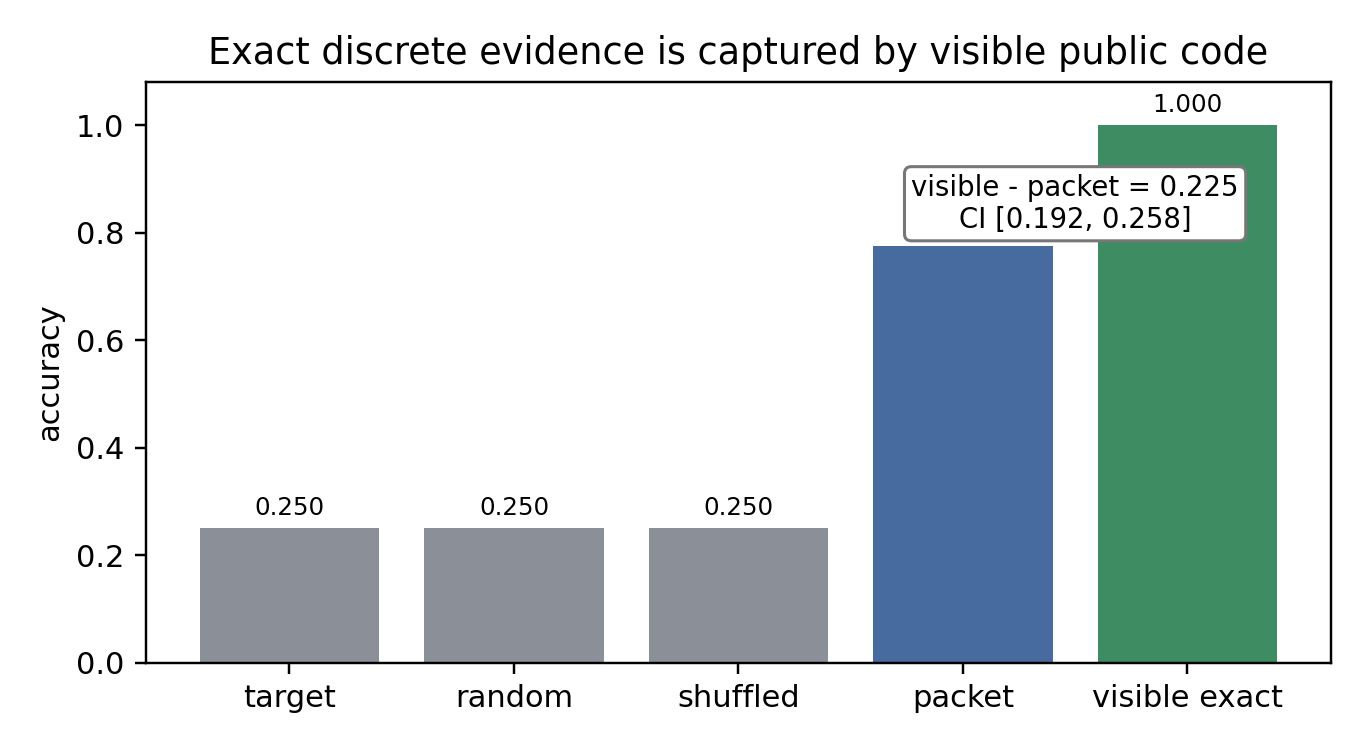
\includegraphics{figures/discrete_evidence_bar.png}
\caption{Exact discrete evidence}
\end{figure}

Figure 3: Cached exact-evidence support: the exact visible public
signature reaches \(1.000\) accuracy, while the learned matched
packet reaches \(0.775\). Controls remain at chance.

The exact-discrete evidence test is the cleanest negative result. The
matched learned packet is useful, but the exact symbolic evidence that
makes it useful is also public-code serializable inside the same byte
budget. When the receiver gets that code visibly, it reaches perfect
accuracy in this cache.

This empirical result has a simple a-priori explanation that makes it
general for its class. A byte-budgeted packet and an equal-byte visible
baseline have the same capacity, natural-language text is a
near-universal code for discrete symbolic content at a given byte
budget, and the receiver is a language model that decodes text natively,
with no learned packet-specific decoder. Consequently, any finite
symbolic evidence signature representable in B bytes can be written as B
bytes of visible text and read by the receiver at least as well. A
learned binary code packs marginally more bits per byte, but only for
payloads that saturate the budget and only after training the receiver
to decode it; neither yields the qualitative beyond-source-choice
advantage the no-text framing seeks. The cached test, visible
\(1.000\) versus packet \(0.775\), is one confirmation. The
argument predicts the dominance holds whenever the useful content is
discrete and equal-byte visible code is permitted.

This is not a universal impossibility theorem. The sample has
\(640\) model-helper rows but only \(160\) unique examples. We
therefore state it as an operational result for this class of evidence,
not as a theorem over all communication protocols.

\hypertarget{the-privacy-bottleneck-escape-does-not-produce-a-privacy-positive-packet}{%
\subsubsection{4.4 the privacy-bottleneck escape Does Not Produce A
Privacy-Positive
Packet}\label{the-privacy-bottleneck-escape-does-not-produce-a-privacy-positive-packet}}

\begin{figure}
\centering
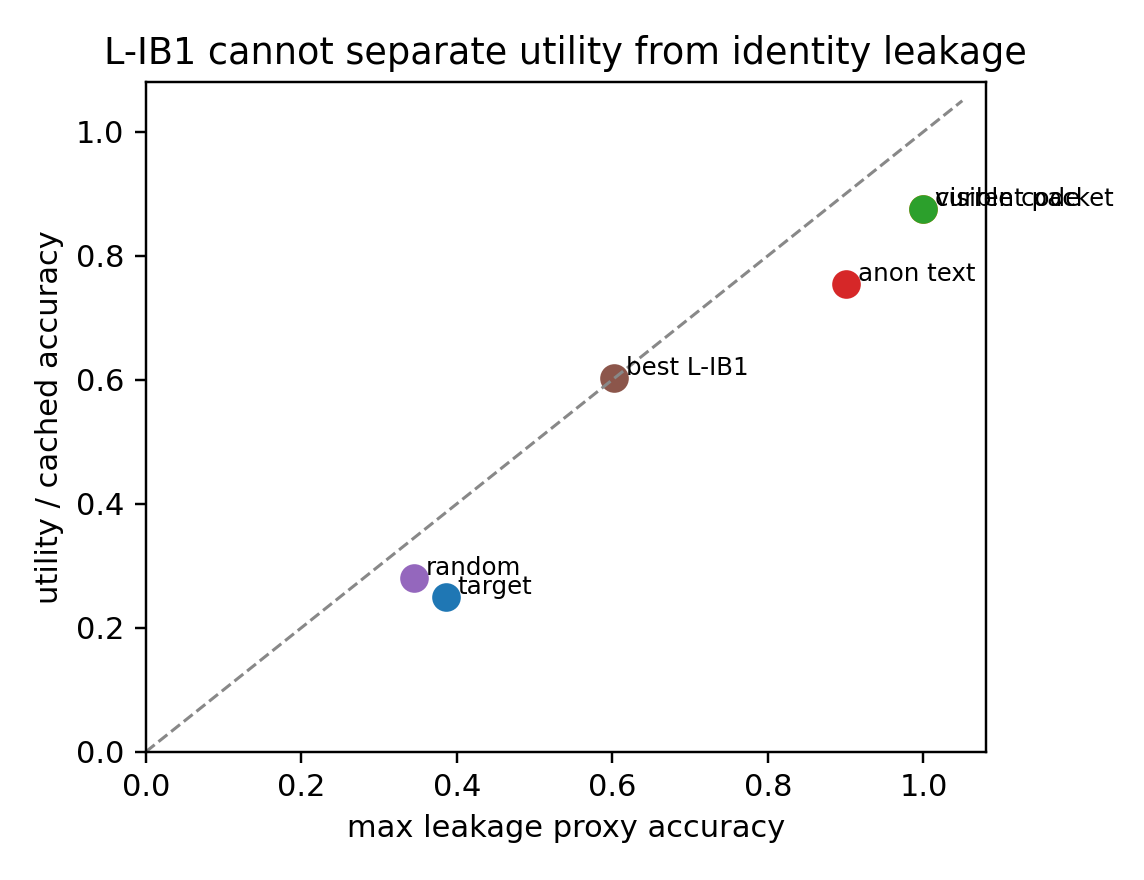
\includegraphics{figures/l_ib_utility_leakage.png}
\caption{the privacy-bottleneck escape utility leakage frontier}
\end{figure}

Figure 4: the privacy-bottleneck escape cannot move off the
utility/leakage identity diagonal enough to preserve utility while
hiding source/evidence structure.

the privacy-bottleneck escape asked whether an adversarial feature
selector could keep utility while hiding source/evidence identity on
\(512\) cached rows. It could not. The current high-utility packet
has cached utility \(0.875\) and max leakage \(1.000\); the
best bottleneck has proxy utility \(0.602339\) and max leakage
\(0.602339\). The exact public code matches current-packet utility
and leakage, while adaptive anonymized text remains a necessary
comparator for any future privacy claim.

The verdict remains utility is identity leakage. This is a
cached gate, not a formal privacy impossibility result. It kills the
cheap local escape and sets the bar for a future build-scale IB method.

\hypertarget{rejected-oracle-ceilings-are-not-communication-claims}{%
\subsubsection{4.5 Rejected Oracle Ceilings Are Not Communication
Claims}\label{rejected-oracle-ceilings-are-not-communication-claims}}

Two large apparent ceilings are explicitly excluded. rerank's strict
rerank oracle and fuser's strict fuser oracle measure answer-aware or
setup-blocked gaps, not deployable no-text communication. The gold-blind
rerank attempt reaches only \(82\) prompts, below its required
floor, and ties the equal-byte text control. fuser has no reviewed
gold-free hidden-state fuser objective locally.

These results are useful only as warnings. A high oracle ceiling does
not imply a latent packet win unless the scorer/fuser is gold-blind and
beats equal-byte text/source-index controls.

\hypertarget{related-work-and-scope}{%
\subsection{5. Related Work And Scope}\label{related-work-and-scope}}

Continuous cache/state communication systems such as C2C
\citep{c2c2026}, KVComm \citep{kvcomm2026}, Interlat
\citep{interlat2026}, and Latent Cache Flow \citep{lcf2026} occupy a
different lane: they transmit or align dense hidden state rather than a
small discrete evidence packet. This paper does not contradict that
dense/cache line of work. It says that, when the message is a low-byte
discrete packet and the useful content is a finite symbolic evidence
signature or score sketch, equal-byte visible evidence and source-index
controls are the correct baseline family.

Adjacent calibrated-routing and structured-communication systems,
including UCCI \citep{ucci2026}, DarkForest \citep{darkforest2026},
structured message passing \citep{smp2013}, and CU-HLM
\citep{cu_hlm2026}, motivate the same hard-baseline discipline: a packet
must beat the visible or routed evidence that an ordinary system could
transmit directly.

Privacy-preserving semantic communication and adaptive text
anonymization motivate the privacy frontier
\citep{ibal2023, adaptive_anonymization2026}. In this paper they
function as baselines and scope limits: a no-text privacy claim must
beat adaptive visible text at the same byte budget while demonstrating
lower leakage.

The closest practical baselines for this work are deliberately simple:
source identity, source confidence, source rank, equal-byte score
sketches, equal-byte visible evidence, wrong-row packets, and shuffled
packets. These baselines are the point. They turn raw helper gains into
deployable communication claims only when the gain survives.

\hypertarget{limitations}{%
\subsection{6. Limitations}\label{limitations}}

The exact-discrete evidence test has \(640\) model-helper rows but
only \(160\) unique examples. The result is strong for this cache
and evidence class, but it is not a theorem over all protocols.

the privacy-bottleneck escape is a CPU cached feature-selector test. It
does not train a live neural encoder, run new generation, or test
continuous dense state.

The held-out one-way result is used as aggregate evidence only. Raw
held-out rows are not packaged, and no paper-finalization step reads or
reruns them.

The paper does not claim that latent communication is impossible. It
claims that the completed byte-scale discrete packet regimes do not
establish a no-text advantage over hard visible/score baselines.

\hypertarget{conclusion}{%
\subsection{7. Conclusion}\label{conclusion}}

LatentWire did not produce a deployable no-text byte-scale positive. It
produced a sharp boundary. Score-like source packets are mostly
redundant after receiver conditioning, exact discrete evidence is better
transmitted as equal-byte visible public code, and the cheap privacy
bottleneck cannot separate utility from identity leakage. Future
positives must leave this killed regime: continuous dense state, or a
real privacy-preserving bottleneck that beats adaptive same-byte text.


\bibliographystyle{../colm2026_conference}
\bibliography{../references}

\end{document}
